\documentclass[12pt,oneside]{article}

% General packages
\usepackage[utf8]{inputenc}
\usepackage{wrapfig}
\usepackage{hyperref}
\hypersetup{
    colorlinks=true,
    linkcolor=black,
    citecolor=red,
    urlcolor=blue
}
\usepackage{siunitx}
%\usepackage[lighttt]{lmodern}

% Geometry package
\usepackage[a4paper,width=150mm,top=30mm,bottom=25mm]{geometry}

% Graphics packages
\usepackage{graphicx}
\graphicspath{img}
\usepackage{float}
\usepackage{amsmath}
\usepackage{listings}
\usepackage{color}

\definecolor{code_numbercolor}{rgb}{0.1, 0.1, 0.8}
\definecolor{code_keywordcolor}{rgb}{0.85, 0.5, 0.05}
\lstset{
    backgroundcolor=\color{white},
    basicstyle=\ttfamily\footnotesize\color{black},
    numberstyle=\ttfamily\tiny\color{black},
    keywordstyle=\ttfamily\bfseries\color{code_keywordcolor},
    breaklines=true,
    numbers=left,
    language=C++,
    morekeywords={string, vector, size_t}
}

% Bibliography
\usepackage[
    backend=biber,
    style=ieee
]{biblatex}

\addbibresource{bibliography.bib}

\newcommand{\githublink}[1]{\href{https://github.com/arscisca/mem-pmod}{#1}}

\title{
	{\Huge \textbf{Politecnico di Torino}}\\ \ \\
	{\large Project for Advanced Design for Signal Integrity and Compliance} \\ \ \\
    {\huge \textbf{A Power Bus-Model for High-Speed Memory Circuits}} \\ \ \\
	{
\includegraphics[width=\textwidth]{img/polito_logo_2021_blu}}
}
\author{
	\textsc{Alessandro Rocco Scisca} \\
    s276032
}
\date{} % Do not insert date


\begin{document}
    \maketitle
    \newpage
    \tableofcontents
    \hypersetup{linkcolor=blue}
    \section{Introduction}
This project is based on the results of the article \emph{A Broadband Chip-Level Power-Bus Model Feasible for Power Integrity Chip-Package Codesign in High-Speed Memory Circuits} \cite{Hao-HsiangChuang2010ABCP}. All the source code and experimental data is publicly available on \href{https://github.com/arscisca/mem-pmod}{GitHub}.

\subsection{Power Integrity}
As for most devices gaining traction both in the consumer oriented and in the general electronics markets, memory systems have been greatly increasing their performance over the past years and newer standards are always proposed for future architectures.

Along with the significant increase in capacity, it is the memory speed -intended as its data transfer rate- which is central in this constant improvement process. Speed is such a crucial parameter because memories are generally much slower than the main processor, meaning that trying to access data may cost a few precious CPU cycles whenever such data is to be read from the main memory (e.g.: not present in caches or local CPU registers). The system will most certainly benefit from a faster memory, but the design process of such high speed memories becomes more and more of concern. Specifically, the chip's Power Integrity has to be well analyzed and taken care of.

Writing data to a bus at such speeds requires not only faster bus drivers, but also a solid internal power bus which may suffer from the constant high frequency, high current switching that is required. Because of the parasitics of the bus, voltage drops and unintended filtering may cause the outputs to be unrecognizable.
This is the reason why it is necessary to study an efficient model for the power bus in order to simulate its behavior at arbitrary frequencies.

    \section{Model}
\subsection{Sections}
Memories are organized so that each output data pin \texttt{DQ} is interleaved with \texttt{VDDQ} and \texttt{VSSQ} power pins as in \autoref{fig:pin-layout} to help the receiver in recognizing the data which may be distorted at such high speeds.
\begin{figure}[htbp]
	\center
	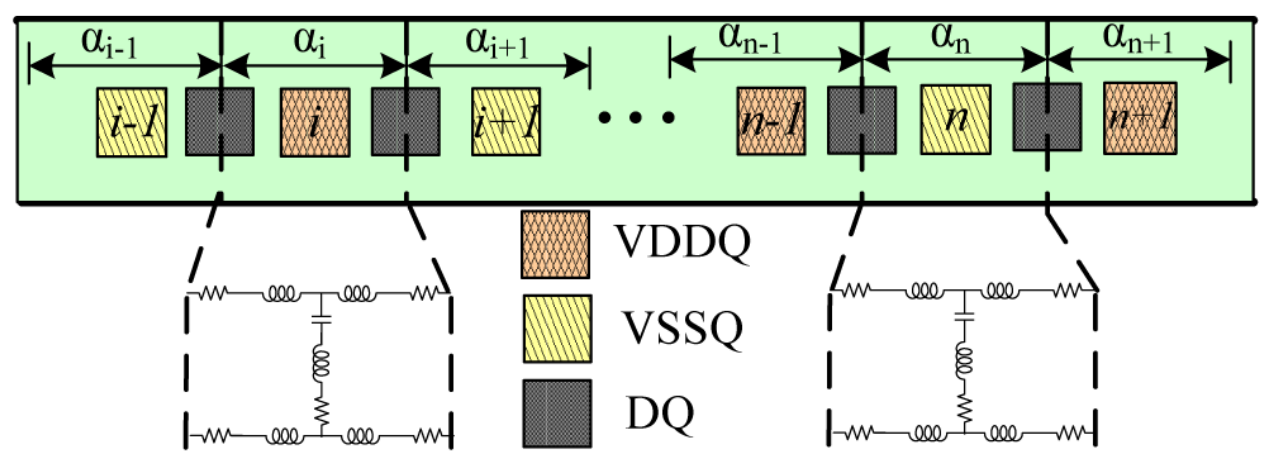
\includegraphics[width = \textwidth]{img/pin-layout}
	\caption{Pin layout of a memory chip}
	\label{fig:pin-layout}
\end{figure}

It is possible to split the power bus in sections - one for each power pin - of lengths $\alpha_i$ as shown in \autoref{fig:pin-layout}. Each section can be modeled with a two port device strucured as in \autoref{fig:tsection-model}.
\begin{figure}[htbp]
	\center
	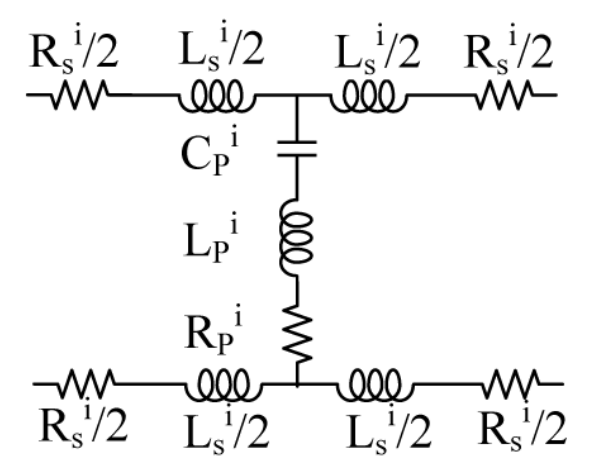
\includegraphics[width = 0.4\textwidth]{img/tsection-model}
	\caption{Model of a single section of a memory output}
	\label{fig:tsection-model}
\end{figure}

\subsection{Parameters}
\label{ssec:parameters}
Each section has five characterizing parameters: $R^i_s$, $L^i_s$, $R^i_p$, $L^i_p$, $C^i_p$ which depend on the overall Per-Unit-Length (PUL) parameters $R_s$, $L_s$, $R_p$, $L_p$, $C_p$ and the section length $\alpha_i$. PUL parameters also take the skin effect into consideration by using a DC resistance and an AC resistance which depends on frequency. The effective resistance of a memory section will be the greatest of the two for a given frequency.

In general, section parameters are computed from PUL parameters with the following formulas:
\begin{align*}
    R^i_s &= \alpha_i \max\left(R_{s,\,dc},\, R_{s,\,ac}\sqrt{\omega}\right) \\
    L^i_s &= \alpha_i L_s \\
    R^i_p &= \frac{1}{\alpha_i} \max\left(R_{p,\,dc},\, R_{p,\,ac}\sqrt{\omega}\right) \\
    L^i_p &= \frac{1}{\alpha_i} L_p \\
    C^i_p &= \alpha_i C_p
\end{align*}
Thanks to these formulas, it is possible to accurately represent the behavior of a power pin based on the power bus PUL parameters and the section lengths.

\subsection{Fitting}
\label{ssec:fitting}
While section lengths are known a-priori from layout information, PUL parameters can instead be determined by fitting real world electrical measurements. The measured quantity is the two port $Z$ matrix between two arbitrary power pins. In order to compare the model to its real world counterpart, the procedure in \autoref{ssec:from-parameters-to-Z-matrix} explains how the $Z$ matrix can be computed from the model parameters.

The fitting process is thus reduced to a multi-variable optimization process, where the unknowns are the PUL parameters and the error to the real world device is to be minimized. The error function $U\left(\vec{p}\right)$ can be expressed as:
\begin{align*}
    U\left(\vec{p}\right) &= \sum_{i = 0}^N \left|| Z_s\left(\vec{p}, f_i\right) - Z_m(f_i) |\right| ^2
\end{align*}
where $\vec{p}$ is a vector representing the device PUL parameters, $N$ is the total number of measured frequencies, $f_i$ is the i-th measured frequency, $Z_s$ is the impedance matrix obtained from the simulation and $Z_m$ is the measured matrix.

\subsection{From PUL Parameters to Z Matrix}
\label{ssec:from-parameters-to-Z-matrix}
In order to obtain $U(\vec{p})$ it is necessary to compute $Z_s\left(\vec{p}, f_i\right)$, which means computing an impedance matrix starting from the model's PUL parameters.
\begin{enumerate}
    \item Compute each section's parameters from PUL parameters as in \autoref{ssec:parameters}
    \item Compute each section's ABCD matrix with
    \begin{equation*}
        \text{ABCD} = \begin{bmatrix}
            1 + z_i y_i   & (z_i y_i + 2) z_i \\
            y_i           & 1 + z_i y_i
        \end{bmatrix}
    \end{equation*}
    where
    \begin{align*}
        z_i &= j \omega L_s^i + R_s^i \\
        y_i &= \frac{j \omega C_p^i}{1 + j\omega R_p^i C_p^i - \omega^2 L_p^i C_p^i}
    \end{align*}
    \item Divide the layout into three groups by cumulating ABCD matrices: before port 1 ($M_1 = \prod_{i = 0} ^ \text{P1} \text{ABCD}_i$), between port 1 and port 2 ($M_2 = \prod_{i = \text{P1}} ^ \text{P2} \text{ABCD}_i$) and after port 2 ($M_1 = \prod_{i = \text{P2}} ^ R \text{ABCD}_i$).

    \item Compute the $Y$ matrix with
    \begin{align*}
        Y(1, 1) &= \frac{M_1(2, 1)}{M_1(2, 2)} + \frac{M_2(2, 2)}{M_2(1, 2)} \\
        Y(1, 2) &= -\frac{1}{M_2(1, 2)} \\
        Y(2, 1) &= Y(1, 2) \\
        Y(2, 2) &= \frac{M_2(1, 1)}{M_2(1, 2)} + \frac{M_3(2, 1)}{M_3(1, 1)}
    \end{align*}
    \item Invert $Y$ to get the desired $Z$ matrix
\end{enumerate}

\subsection{Results}
After finding the best $\vec{p}$ that minimizes $U(\vec{p})$, the resulting PUL parameters are a good description of the physical device which limits the model error. The simulation ran from the author returns the results shown in \autoref{fig:zmatrix-paper}, which show how close the simulation is to the actual measurements.

\begin{figure}[htbp]
    \center
    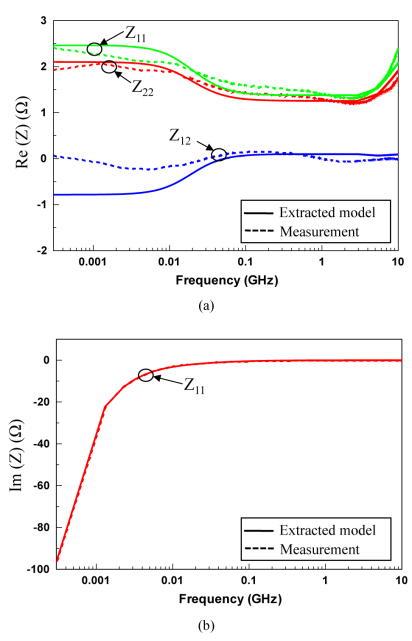
\includegraphics[width = 0.4\textwidth]{img/zmatrix-paper}
    \caption{Results from paper}
    \end{figure}
    \label{fig:zmatrix-paper}

    \section{Implementation}
The presented model is very simple yet shows a good accuracy on a wide band of frequencies. A possible improvement on the original discussion is the performance of its implementation. The original implementation is not publicly available, but it is reported that \textit{`the computation time is about 5 minutes at a quad core computer'}\cite{Hao-HsiangChuang2010ABCP} on a MATLAB script\autocite{5451081}.

This proposed implementation, titled \textbf{mem-pmod} (MEMory-PowerMODel) is \githublink{open source} and based on C++ plus the support of Python to generate graphics. It aims at a better performance and a higher degree of reusability. The developed program can simulate and extract a model on the same amount of data in about 50 s, or one sixth of the original amount of time.

\subsection{Features and Organization}
Mem-pmod is developed in C++ and is focused on the optimization of the process. It uses multithreading together with the highly optimized Eigen library to maximize performance. It offers:
\begin{itemize}
    \item Memory model fitting to experimental data as described from the paper
    \item Possibility to implement any generic fitting algorithm
    \item Model exporting and importing
\end{itemize}
It also includes some testing based on the GTest framework to check some of the available mechanisms.

\autoref{fig:program-flow} shows a typical flow of execution with the supported features.
\begin{figure}[htbp]
    \center
    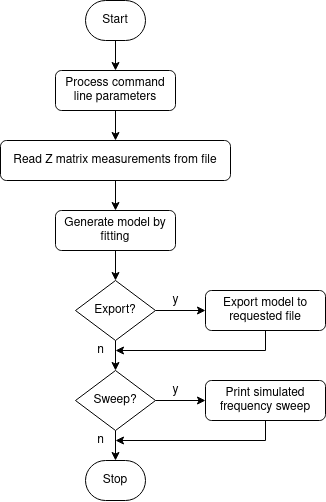
\includegraphics[width = 0.4\textwidth]{img/program-flowchart}
    \caption{Execution flow}
    \label{fig:program-flow}
\end{figure}
The program is organized in modules which may be grouped in three categories:
\begin{itemize}
    \item Models, which offer the infrastructure to build and interact with models
    \item Optimization, used by models to treat the fitting process as a generic optimization problem
    \item General control, which control the flow of the program and also offer some helpful, general purpose structures and functions
\end{itemize}

\subsection{Reading Measurements}
The measurements to be used as fitting data are stored in a text file and passed to the program as a command line parameter. Below is an example of a measurements file.
\begin{lstlisting}[backgroundcolor=\color{white},basicstyle=\tiny,breaklines=true]
f Z11 Z12 Z21 Z22
+1.000000e+06 (+1.253488e+01,-3.163626e+01) (-4.890959e+00,-2.934532e+01) (-4.890959e+00,-2.934532e+01) (+1.253488e+01,-3.163626e+01)
+1.047129e+06 (+1.251280e+01,-3.031854e+01) (-4.869922e+00,-2.792886e+01) (-4.869922e+00,-2.792886e+01) (+1.251280e+01,-3.031854e+01)
+1.096478e+06 (+1.248878e+01,-2.906428e+01) (-4.847045e+00,-2.657249e+01) (-4.847045e+00,-2.657249e+01) (+1.248878e+01,-2.906428e+01)
+1.148154e+06 (+1.246268e+01,-2.787069e+01) (-4.822186e+00,-2.527343e+01) (-4.822186e+00,-2.527343e+01) (+1.246268e+01,-2.787069e+01)
+1.202264e+06 (+1.243432e+01,-2.673511e+01) (-4.795195e+00,-2.402906e+01) (-4.795195e+00,-2.402906e+01) (+1.243432e+01,-2.673511e+01)
\end{lstlisting}
Each line contains, in order, the measurement frequency in Hz and the four elements of the $Z$ matrix in $\Omega$ separated by spaces. Each matrix element is a complex number and it is written as (\textit{real part}, \textit{imaginary part}).

Inside the program, measurements are stored in a specific structure:
\begin{lstlisting}[language=C++]
struct Measurements {
    std::vector<double> frequencies;
    std::vector<Matrix2> Z;
    unsigned port1;
    unsigned port2;
    std::size_t nsamples;
};
\end{lstlisting}
Which is initialized by the function
\begin{lstlisting}
Measurements readMeasurements(const std::string &fname, unsigned port1, unsigned port2);
\end{lstlisting}
The two ports from which the measurements were taken are specified as command line arguments.

\subsection{Geometric and Complete Models}
The overall memory is modeled in two structures: there is a model for a single TSection and a MemoryModel whoch holds an array of TSections plus the PUL parameters. There is a distinction between Geometric and Complete models: geometric models only keep track of geometry information, complete models also contain electrical parameters and additional information. Below are some snippets of the various models in their two forms:

\begin{lstlisting}[title=Snippets for Geometric and Complete TSection]
class GeometricTSection {
public:
    GeometricTSection();
    ...
protected:
    double _length;
};

class TSection : private GeometricTSection {
public:
    TSection();
    ...
private:
    LumpedParameters _parameters;
};
\end{lstlisting}

\begin{lstlisting}[title=Snippets for Geometric and Complete MemoryModel]
template <std::size_t NPowerPorts>
class GeometricMemoryModel {
public:
    GeometricMemoryModel();
    ...
private:
    std::array<GeometricTSection, NPowerPorts> _sections;
};

template<std::size_t NPowerPorts>
class MemoryModel : private GeometricMemoryModel<NPowerPorts> {
public:
    MemoryModel();
    ...
private:
    std::array<TSection, NPowerPorts> _sections;
    PULParameters _pul_parameters;
};
\end{lstlisting}

\subsection{Fitting}
The MemoryModel class also offers the interface for fitting and this is where multithreading happens. This class offers a static method called \texttt{fit()} to initialize a model by fitting measurements using the optimization module.
\begin{lstlisting}
static MemoryModel<NPowerPorts> fit(
        const Measurements &measurements,
        const std::array<double, NPowerPorts> lengths,
        pmod::optimization::Algorithm method = pmod::optimization::Algorithm::CDESCENT);
\end{lstlisting}
The function \texttt{fittingError()}, also offered from the same class, is the function that computes the error function described in \autoref{ssec:fitting} of a given model. This function is very expensive because it computes the Z matrix of a model for each measured frequency, but luckily this process can be parallelized with multithreading by splitting the job in chunks, each handled by a thread. The number of threads depends on hardware information in order to always maximize performance.
\begin{lstlisting}
static double fittingError(
            const GeometricMemoryModel<NPowerPorts> &model,
            const PULParameters &pul_parameters,
            const Measurements &measurements,
            bool enable_threading = true)
\end{lstlisting}

The optimization module is the one that runs the actual optimization algorithm and it treats everything as a generic multidimensional optimization problem. It offers the templated function
\begin{lstlisting}
template<std::size_t N>
Vector<N> optimize(Algorithm algorithm, std::function<double(Vector<N>)> function, Vector<N> x0, double threshold);
\end{lstlisting}
which automatically manages everything and allows for the choice of an optimization algorithm.

The original paper uses Powell's method whose manual implementation is difficult and outside the current scope of this project. The currently implemented algorithm is a modified version of the Coordinate Descent algorithm, which can be slower and may get trapped in local minima more easily. The algorithm simply minimizes the function along each dimension in turn.
\begin{figure}[htbp]
    \center
    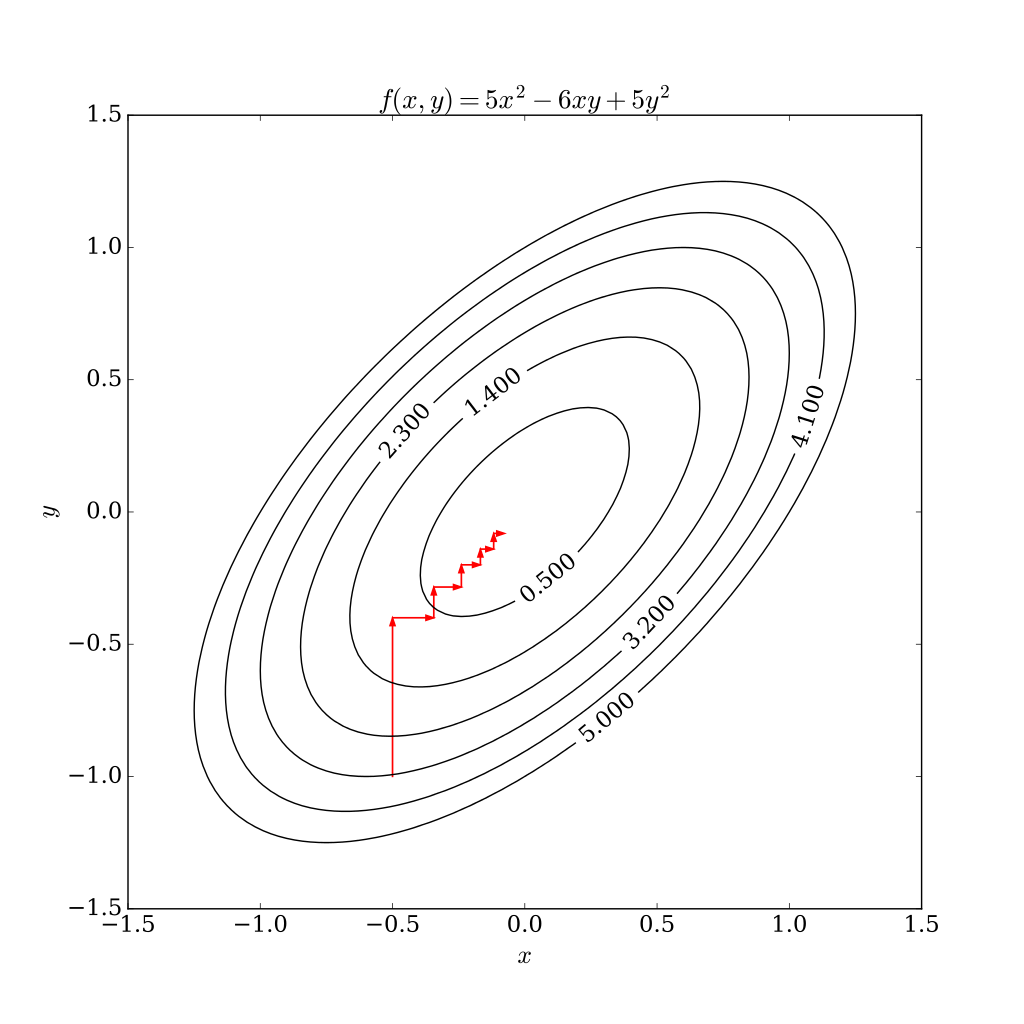
\includegraphics[width = 0.7\textwidth]{img/coordinate_descent}
    \caption{Behavior of the Coordinate Descent algorithm. Courtesy of Wikipedia\autocite{CoordinateDescent}}
    \label{fig:example-output}
\end{figure}
In order to minimize the likelihood of getting trapped in local minima, the algorithm detects when stability is reached too soon and, in that case, adds some noise to free the point from the trap. The best minimum is always recorded and it is the one that is returned as a result.

\subsection{Importing and Exporting}
As mentioned above, it is also possible to import and export memory models. This is done by specific functions implemented for the MemoryModel and TSection classes which internally manage all the necessary steps. The current implementation simply dumps all the relevant parameters in order in a text file and then the importer just reads them.

\subsection{Results}
The results discussed in this section will be numerically different from the ones of the paper, but it is evident how the trend is perfectly matching. This is because:
\begin{enumerate}
    \item Measurements used in the paper are not available nor easily accessible, so they were manually generated
    \item The paper only specifies the overall memory length ($\SI{4074}{\micro m}$), so it was assumed all sections were equally long. This assumption is likely imprecise
    \item The optimization algorithm is different
\end{enumerate}
In any case, everything was set up to be as reasonably close as possible to the the results from the paper and to realistic values.

\begin{figure}[htbp]
    \center
    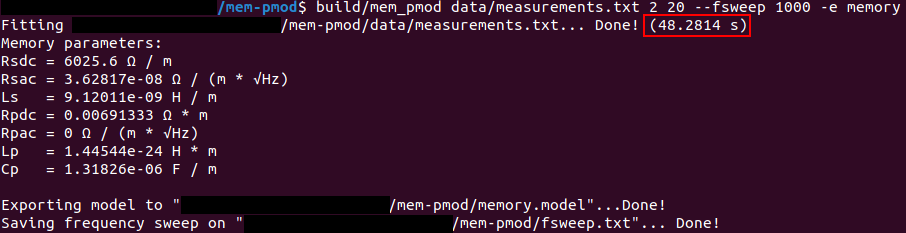
\includegraphics[width = \textwidth]{img/example_output}
    \caption{Example execution of mem-pmod. Execution time is highlighted in red.}
    \label{fig:example-output}
\end{figure}
\autoref{fig:example-output} shows what a typical execution of mem-pmod looks like. The command line parameters specify, in order: the measurements file, the measurements ports, request a frequency sweep simulation with 1000 frequency samples (from 1 MHz to 10 GHz) and to export the model to a file called \texttt{memory.model}. There was a total of 1000 measurement points in this run, the same amount as were used in the original paper.
\begin{table}[htbp]
    \center
    \begin{tabular}{|l|l|l|}
        \hline
        Quantity & Value \\ \hline
        Rsdc & $\SI{5312.13}{\Omega / m}$ \\ \hline
        Rsac & $\SI{0.0238141}{\Omega / (m * \sqrt{Hz})}$ \\ \hline
        Ls   & $\SI{9.18165e-09}{H / m}$ \\ \hline
        Rpdc & $\SI{0.00695145}{\Omega * m}$ \\ \hline
        Rpac & $\SI{1e-38}{\Omega / (m * \sqrt{Hz})}$ \\ \hline
        Lp   & $\SI{4.74466e-28}{H / m}$ \\ \hline
        Cp   & $\SI{1.31426e-06}{F / m}$ \\ \hline
    \end{tabular}
    \caption{Resulting PUL parameters from mem-pmod}
    \label{tab:pul-parameters}
\end{table}
The obtained PUL parameters visible in \autoref{fig:example-output} are also shown in \autoref{tab:pul-parameters} for clarity. Finally, the obtained frequency sweep is matched against the original measurements with the help of a Python script and the matplotlib library. The results of this comparison are shown in \autoref{fig:zmatrix}.

\begin{figure}[htbp]
    \center
    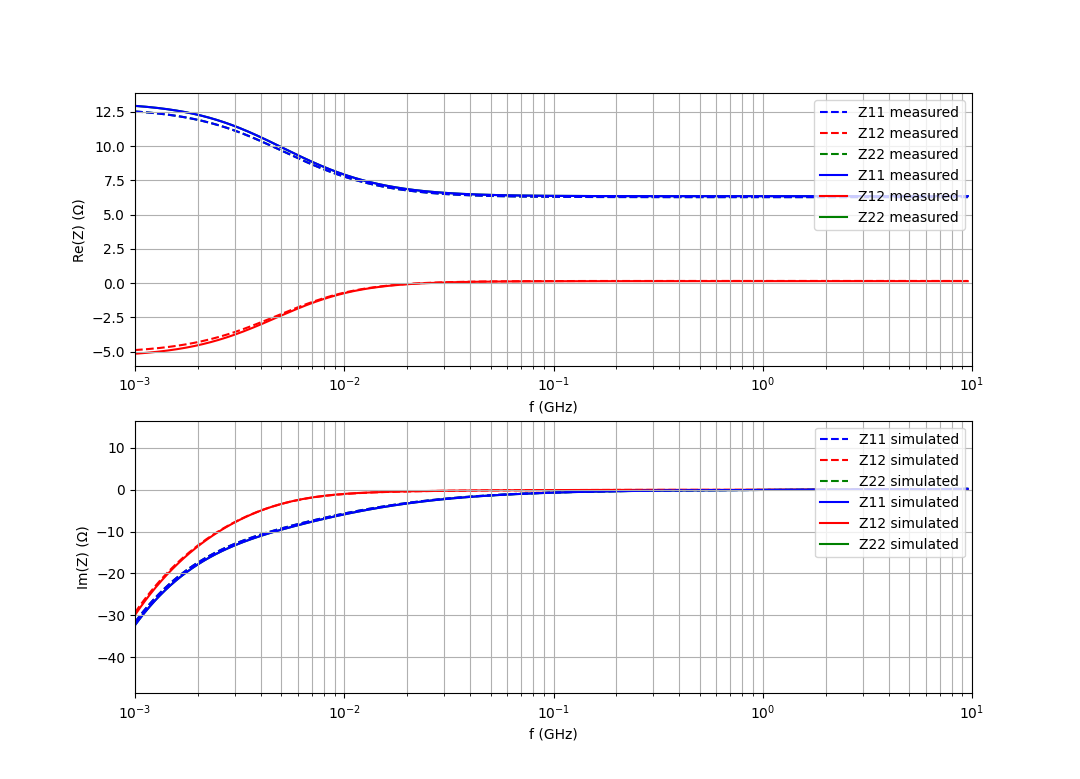
\includegraphics[width = \textwidth]{img/zmatrix}
    \caption{Results from mem-pmod against passed measurements}
    \label{fig:zmatrix}
\end{figure}


Comparing \autoref{fig:zmatrix} to \autoref{fig:zmatrix-paper}, the one generated from the researchers, shows how even though the numerical values differ the general behavior is the same.

    \printbibliography[heading=bibintoc]
\end{document}
